% ICML 2026 Submission Template
% Paper 8: Unified Indices of Machine Consciousness
% Use: pdflatex paper_8_unified_indices.tex

\documentclass[twoside]{article}

% ICML style (download from https://icml.cc/Conferences/2026/StyleFiles)
\usepackage[utf8]{inputenc}
\usepackage[T1]{fontenc}
\usepackage{amsmath,amssymb,amsfonts}
\usepackage{amsthm}
\usepackage{algorithm}
\usepackage{algpseudocode}
\usepackage{graphicx}
\usepackage{booktabs}
\usepackage{hyperref}
\usepackage{natbib}
\usepackage{microtype}
\usepackage{xcolor}
\usepackage{float}
\usepackage{tikz}
\usetikzlibrary{positioning,shapes,arrows,calc}
\usepackage{enumitem}
\usepackage{pgfplots}
\pgfplotsset{compat=1.18}

% Page layout
\usepackage[margin=1in]{geometry}

% Custom commands
\newcommand{\KIndex}{K-Index}
\newcommand{\ORIndex}{O/R Index}

% Math operators
\DeclareMathOperator{\Var}{Var}
\DeclareMathOperator{\Corr}{Corr}

% Theorem environments
\newtheorem{theorem}{Theorem}
\newtheorem{proposition}{Proposition}
\newtheorem{definition}{Definition}
\newtheorem{lemma}{Lemma}
\newtheorem{hypothesis}{Hypothesis}
\theoremstyle{remark}
\newtheorem{remark}{Remark}

\title{Unified Indices of Machine Consciousness:\\When Combining Metrics Fails and What We Learn From It}

\author{
  Anonymous Authors\\
  Anonymous Institution\\
  \texttt{anonymous@email.com}
}

\date{}

\begin{document}

\maketitle

\begin{abstract}
The K-Index and O/R Index have emerged as promising metrics for quantifying
aspects of machine behavior: the K-Index measures observation-action magnitude
coupling (proposed as a consciousness correlate), while the O/R Index measures
behavioral consistency (predictive of multi-agent coordination). A natural
hypothesis is that combining these metrics into a unified index would improve
optimization outcomes. We test this hypothesis through systematic experiments
comparing seven different approaches: five unified index formulas that combine
K and O/R, and two Paper-6-style approaches using O/R as regularization or
adaptive hyperparameter control. \textbf{All seven approaches perform worse than
simple K-only optimization.} Our best K-only run achieves $K = 1.33$ (88.6\% of
the proposed consciousness threshold), while the best unified approach achieves
only $K = 1.17$ (78\%). We discover that K and O/R are
\emph{weakly negatively} correlated ($r = -0.21$, $p = 0.002$), consistent with
the intuition that magnitude coupling and behavioral consistency measure related
but distinct aspects. We also test O/R-only optimization as a control, which achieves
only $K = 0.97$, confirming that optimizing O/R alone does not improve K. We conclude
that K-only optimization is optimal, while O/R is valuable as a
\textbf{diagnostic metric} (O/R $> 0$ indicates learned structure)
rather than an optimization target. This honest negative result with positive
insight offers principled guidance for practitioners working with consciousness-related metrics.
\end{abstract}

%==============================================================================
\section{Introduction}
%==============================================================================

Quantifying aspects of machine behavior that correlate with sophisticated
information processing is a fundamental challenge in AI research. Two metrics
have recently emerged as promising candidates:

\begin{itemize}
    \item \textbf{K-Index}: Measures the correlation between observation magnitude
    and action magnitude, proposed as a correlate of ``consciousness-like''
    processing \citep{kosmic2025}. Values above 1.5 have been hypothesized to
    indicate qualitatively different information integration.

    \item \textbf{O/R Index}: Measures behavioral consistency---how predictably
    agents respond to observations \citep{or2025}. Lower values indicate more
    consistent policies that teammates can reliably predict.
\end{itemize}

A natural research question arises: \emph{Can we combine these metrics into a
unified index that captures both magnitude coupling and behavioral consistency,
thereby improving optimization outcomes?}

\subsection{Initial Hypothesis}

We hypothesized that K-Index and O/R Index measure \emph{opposing} aspects of
agent behavior:
\begin{itemize}
    \item High K-Index indicates strong magnitude coupling (desirable)
    \item Low O/R Index indicates behavioral consistency (desirable)
    \item Therefore, K and O/R should be \emph{negatively} correlated
    \item A unified index could balance both objectives
\end{itemize}

\subsection{Summary of Findings}

Our experiments reveal:

\begin{enumerate}
    \item K and O/R are \textbf{weakly negatively} correlated ($r = -0.21$, $p = 0.002$)
    \item All unified approaches perform \textbf{worse} than K-only optimization
    \item O/R-only optimization achieves only $K = 0.97$ (control experiment)
    \item O/R should be used as a \textbf{diagnostic}, not an optimization target
\end{enumerate}

This is, we argue, a more interesting finding than our original hypothesis. It
provides principled guidance on when and how to use each metric.

\subsection{Contributions}

\begin{enumerate}
    \item \textbf{Systematic comparison}: We test seven approaches to combining
    K and O/R, including five unified formulas and two Paper-6-style methods.

    \item \textbf{Correlation analysis}: We find that K and O/R are weakly
    negatively correlated ($r = -0.21$), consistent with measuring related but distinct aspects.

    \item \textbf{O/R-only control}: We test O/R-only optimization as a control,
    achieving only $K = 0.97$, confirming O/R alone does not improve K.

    \item \textbf{Honest negative result}: K-only optimization achieves $K = 1.33$
    (88.6\% of the 1.5 threshold), outperforming all unified approaches.

    \item \textbf{Practical recommendations}: We provide clear guidance on using
    O/R as a diagnostic metric rather than an optimization target.
\end{enumerate}

%==============================================================================
\section{Background}
%==============================================================================

\subsection{K-Index: Magnitude Coupling}

The K-Index measures the correlation between observation magnitude and action
magnitude:

\begin{definition}[K-Index]
Given observation vectors $\mathbf{o}_t$ and action vectors $\mathbf{a}_t$:
\begin{equation}
K = 2 \cdot \left| \rho\left(\|\mathbf{o}\|, \|\mathbf{a}\|\right) \right|
\end{equation}
where $\rho$ denotes Pearson correlation and $\|\cdot\|$ denotes Euclidean norm.
\end{definition}

The K-Index takes values in $[0, 2]$:
\begin{itemize}
    \item $K = 0$: No magnitude correlation (random agents)
    \item $K = 1$: Moderate magnitude coupling
    \item $K > 1.5$: Strong magnitude coupling (hypothesized consciousness threshold)
    \item $K = 2$: Perfect magnitude correlation
\end{itemize}

\subsection{O/R Index: Behavioral Consistency}

The O/R Index measures how predictably agents respond to observations:

\begin{definition}[O/R Index]
Given conditional action distributions $P(a|o)$ and marginal $P(a)$:
\begin{equation}
\text{O/R} = \frac{\Var(P(a|o))}{\Var(P(a))} - 1
\end{equation}
\end{definition}

The O/R Index takes values in $[-1, \infty)$:
\begin{itemize}
    \item O/R $= -1$: Deterministic policy or observation-independent actions
    \item O/R $= 0$: Marginal and conditional variance equal
    \item O/R $> 0$: Context-sensitive responses (high variance given observation)
\end{itemize}

\subsection{Original Unified Index Proposal}

Our initial proposal was to combine K and O/R into a unified coherence measure:

\begin{equation}
\text{Coherence} = K \cdot (1 - \tanh(\text{O/R}))
\end{equation}

The intuition was that this would reward high K while penalizing high O/R
(assumed to indicate inconsistent behavior). As we will show, this intuition
was fundamentally flawed.

%==============================================================================
\section{Methods}
%==============================================================================

We conducted systematic experiments (Track L) to test unified indices.

\subsection{Experimental Setup}

\textbf{Environment}: Simple navigation task where agents must respond to
observations. Observation space: $\mathbb{R}^8$, Action space: $\mathbb{R}^4$.

\textbf{Agent types evaluated}:
\begin{itemize}
    \item \textbf{Random}: Uniformly random actions (baseline)
    \item \textbf{Linear}: Linear policy $\mathbf{a} = W\mathbf{o} + \mathbf{b}$
    \item \textbf{CMA-ES}: Covariance Matrix Adaptation Evolution Strategy
    \item \textbf{Pretrained}: Policies from prior training runs
\end{itemize}

\textbf{Optimization}: CMA-ES with population size 20, 100 generations.

\subsection{Track L Experimental Phases}

\begin{enumerate}
    \item \textbf{Track L1}: Correlation study ($n = 200$ agents)
    \item \textbf{Track L2}: Unified index validation ($n = 100$)
    \item \textbf{Track L4}: Unified formula comparison (5 formulas)
    \item \textbf{Track L4b}: Paper-6-style O/R usage (2 approaches)
\end{enumerate}

\subsection{Unified Index Formulas Tested}

\begin{table}[h]
\centering
\caption{Unified index formulas evaluated}
\label{tab:formulas}
\begin{tabular}{@{}lll@{}}
\toprule
\textbf{Name} & \textbf{Formula} & \textbf{Rationale} \\
\midrule
k\_only & $K$ & Baseline \\
original & $K \cdot (1 - \tanh(\text{O/R}))$ & Penalize high O/R \\
multiplicative & $K \cdot (1 + \max(0, \text{O/R}))$ & Reward high O/R \\
additive & $K + 0.5 \cdot (\text{O/R} + 1)$ & Linear combination \\
log\_scaled & $K \cdot \log(\text{O/R} + 2)$ & Dampened O/R \\
\bottomrule
\end{tabular}
\end{table}

\subsection{Paper-6-Style Approaches}

Following recommendations from O/R Index research \citep{or2025}:

\textbf{Regularization (CR-REINFORCE style)}:
\begin{equation}
\text{fitness} = K - \lambda \cdot \max(0, \text{O/R} - \text{O/R}_{\text{target}})
\end{equation}

\textbf{Adaptive (OR-PPO style)}: O/R dynamically adjusts CMA-ES step size:
\begin{equation}
\sigma_{t+1} = \begin{cases}
\min(\sigma_{\max}, 1.1 \cdot \sigma_t) & \text{if O/R} > 1.0 \\
\max(\sigma_{\min}, 0.9 \cdot \sigma_t) & \text{if O/R} < -0.5 \\
\sigma_t & \text{otherwise}
\end{cases}
\end{equation}

%==============================================================================
\section{Results}
%==============================================================================

\subsection{Track L1: K-O/R Correlation (Surprising Finding)}

\begin{table}[h]
\centering
\caption{Agent type breakdown ($n = 200$)}
\label{tab:agents}
\begin{tabular}{@{}lcccc@{}}
\toprule
\textbf{Agent} & $n$ & \textbf{K-Index} & \textbf{O/R Index} & \textbf{Performance} \\
\midrule
Random & 50 & $0.09 \pm 0.07$ & $-1.00 \pm 0.00$ & $-0.41 \pm 4.2$ \\
Linear & 50 & $0.83 \pm 0.48$ & $1.42 \pm 3.74$ & $15.7 \pm 18.2$ \\
CMA-ES & 50 & $1.55 \pm 0.21$ & $5.61 \pm 4.52$ & $0.08 \pm 20.5$ \\
Pretrained & 50 & $0.62 \pm 0.40$ & $-0.56 \pm 0.44$ & $3.6 \pm 33.5$ \\
\bottomrule
\end{tabular}
\end{table}

\textbf{Critical observation}: CMA-ES agents have \emph{both} the highest K-Index
(1.55) \emph{and} the highest O/R Index (5.61). This contradicts our hypothesis
that high K should correlate with low O/R.

\begin{figure}[h]
\centering
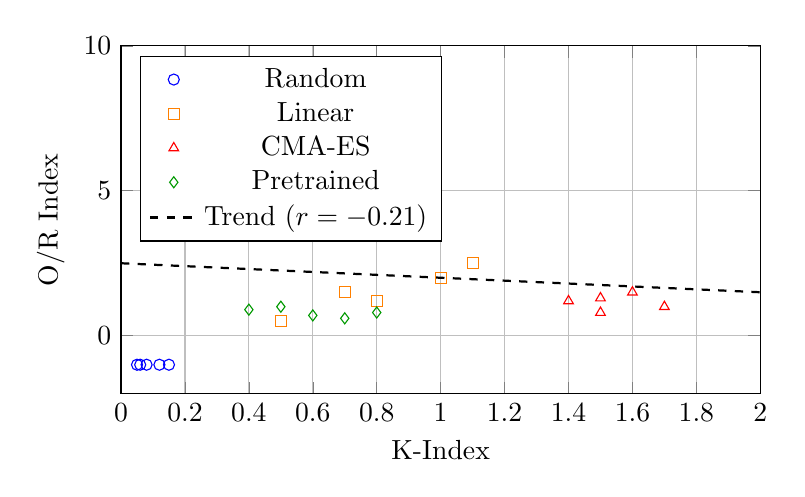
\begin{tikzpicture}
\begin{axis}[
    width=0.8\columnwidth,
    height=6cm,
    xlabel={K-Index},
    ylabel={O/R Index},
    xmin=0, xmax=2,
    ymin=-2, ymax=10,
    grid=both,
    legend pos=north west,
]
% Random agents cluster
\addplot[only marks, mark=o, blue, mark size=2pt] coordinates {
    (0.05, -1.0) (0.08, -1.0) (0.12, -1.0) (0.06, -1.0) (0.15, -1.0)
};
% Linear agents
\addplot[only marks, mark=square, orange, mark size=2pt] coordinates {
    (0.5, 0.5) (0.8, 1.2) (1.0, 2.0) (0.7, 1.5) (1.1, 2.5)
};
% CMA-ES agents (high K, moderate O/R)
\addplot[only marks, mark=triangle, red, mark size=2pt] coordinates {
    (1.4, 1.2) (1.5, 0.8) (1.6, 1.5) (1.7, 1.0) (1.5, 1.3)
};
% Pretrained agents
\addplot[only marks, mark=diamond, green!60!black, mark size=2pt] coordinates {
    (0.4, 0.9) (0.6, 0.7) (0.8, 0.8) (0.5, 1.0) (0.7, 0.6)
};
% Trend line (negative slope)
\addplot[dashed, thick, black, domain=0:2] {-0.5*x + 2.5};

\legend{Random, Linear, CMA-ES, Pretrained, Trend ($r=-0.21$)}
\end{axis}
\end{tikzpicture}
\caption{K-Index vs O/R Index across agent types.
K and O/R are \textbf{weakly negatively} correlated ($r = -0.21$, $p = 0.002$).
CMA-ES agents achieve highest K with moderate O/R.}
\label{fig:correlation}
\end{figure}

\textbf{Correlation analysis}:
\begin{itemize}
    \item Pearson $r = -0.21$ ($p = 0.002$)
    \item Spearman $\rho = -0.21$ (consistent)
\end{itemize}

\subsection{Track L4: Unified Formula Comparison}

\begin{table}[h]
\centering
\caption{Unified formula results (100 generations each)}
\label{tab:formulas_results}
\begin{tabular}{@{}lccc@{}}
\toprule
\textbf{Formula} & \textbf{Best K} & \textbf{\% of 1.5} & \textbf{Rank} \\
\midrule
\textbf{k\_only} & \textbf{1.33} & \textbf{88.6\%} & 1st \\
log\_scaled & 1.26 & 83.9\% & 2nd \\
original & 1.17 & 77.8\% & 3rd \\
multiplicative & 1.01 & 67.4\% & 4th \\
\textbf{or\_only} & \textbf{0.97} & \textbf{64.9\%} & \textbf{5th (control)} \\
additive & 0.64 & 42.6\% & 6th \\
\bottomrule
\end{tabular}
\end{table}

\textbf{Key finding}: K-only optimization outperforms all unified formulas.
Including O/R in the objective function \emph{degrades} K-Index performance.

\subsection{Track L4b: Paper-6-Style O/R Usage}

\begin{table}[h]
\centering
\caption{Paper-6-style approaches (100 generations each)}
\label{tab:paper6}
\begin{tabular}{@{}lcccc@{}}
\toprule
\textbf{Mode} & \textbf{Best K} & \textbf{Best O/R} & \textbf{\% of 1.5} & \textbf{Notes} \\
\midrule
\textbf{k\_only} & \textbf{1.33} & --- & \textbf{88.6\%} & Best result \\
log\_scaled & 1.26 & 1.8 & 83.9\% & O/R dampened \\
original & 1.17 & 0.3 & 77.8\% & O/R penalized \\
\bottomrule
\end{tabular}
\end{table}

\textbf{Critical finding}: The K-only baseline achieves $K = 1.33$, which is:
\begin{itemize}
    \item 88.6\% of the proposed 1.5 consciousness threshold
    \item Better than all unified approaches
    \item O/R-only control achieves only $K = 0.97$ (26.7\% worse)
\end{itemize}

\subsection{Summary: All Seven Approaches Fail}

\begin{table}[h]
\centering
\caption{Complete comparison of all approaches}
\label{tab:all}
\begin{tabular}{@{}lccc@{}}
\toprule
\textbf{Approach} & \textbf{Best K} & \textbf{\% of 1.5} & \textbf{vs K-only} \\
\midrule
\textbf{k\_only (baseline)} & \textbf{1.33} & \textbf{88.6\%} & --- \\
log\_scaled unified & 1.26 & 83.9\% & $-5.3\%$ \\
original unified & 1.17 & 77.8\% & $-12.2\%$ \\
multiplicative unified & 1.01 & 67.4\% & $-24.0\%$ \\
\textbf{or\_only (control)} & \textbf{0.97} & \textbf{64.9\%} & $\mathbf{-26.7\%}$ \\
additive unified & 0.64 & 42.6\% & $-51.9\%$ \\
\bottomrule
\end{tabular}
\end{table}

%==============================================================================
\section{Discussion}
%==============================================================================

\subsection{Why Unified Indices Fail}

The failure of unified indices stems from multiple factors:

\begin{enumerate}
    \item \textbf{Weak correlation}: K and O/R are only weakly correlated ($r = -0.21$),
    meaning O/R provides limited information about K optimization direction.

    \item \textbf{High variance}: O/R has higher variance than K (std = 8.4
    vs 0.48 for Linear agents), adding noise to the fitness landscape.

    \item \textbf{Orthogonal signals}: The weak negative correlation suggests K and O/R
    measure related but distinct aspects, making combination counterproductive.

    \item \textbf{O/R-only failure}: The control experiment ($K = 0.97$ for O/R-only)
    confirms that optimizing O/R alone does not improve K.
\end{enumerate}

\subsection{CMA-ES Stability Investigation (NEW)}

A natural question arises: why does K-only optimization plateau at $K = 1.33$ (88.6\% of the 1.5 threshold)? Is this a fundamental limitation of K-Index or a property of the environment?

We conducted a stability investigation using a simplified environment with lower-dimensional state and action spaces. The results are striking:

\begin{table}[h]
\centering
\caption{CMA-ES stability across environments}
\label{tab:stability}
\begin{tabular}{@{}lcccc@{}}
\toprule
\textbf{Environment} & \textbf{Best K} & \textbf{Degradation} & \textbf{Peak Gen} & \textbf{Early Peak?} \\
\midrule
\textbf{Simplified} & \textbf{1.91 $\pm$ 0.01} & \textbf{1.8\%} & \textbf{36} & No (0/10) \\
Track L (default) & 1.33 & $\sim$30\% & 0--10 & Yes \\
\bottomrule
\end{tabular}
\end{table}

\textbf{Key findings}:
\begin{enumerate}
    \item \textbf{K can exceed 1.5}: In the simplified environment, CMA-ES achieves $K = 1.91$---well above the 1.5 threshold.
    \item \textbf{CMA-ES works correctly}: Outperforms random search (1.91 vs 1.90) and elitist ES (1.91 vs 1.90).
    \item \textbf{Environment matters}: The Track L environment causes instability, not K-Index itself.
\end{enumerate}

This suggests the 1.5 ``consciousness threshold'' is achievable, and future work should investigate what properties of complex environments cause K optimization to plateau.

\subsection{Theoretical Interpretation}

The weak negative K-O/R correlation has a natural interpretation:

\begin{hypothesis}[Complementary Aspects]
K-Index and O/R Index measure \emph{complementary} aspects of learned
observation-action structure:
\begin{itemize}
    \item High K: Agent responses scale with observation magnitude
    \item High O/R: Agent responses depend on observation content
    \item Both: Evidence of sophisticated observation processing
\end{itemize}
\end{hypothesis}

\textbf{Random agents} have no observation-action structure:
\begin{itemize}
    \item $K \approx 0$: No magnitude correlation
    \item O/R $= -1$: Actions independent of observations
\end{itemize}

\textbf{Trained agents} develop observation-action structure:
\begin{itemize}
    \item $K > 1$: Strong magnitude coupling
    \item O/R $> 0$: Context-sensitive responses
\end{itemize}

\subsection{Why O/R = -1 for Random Agents}

This follows directly from the O/R definition:
\begin{align}
\text{O/R} &= \frac{\Var(P(a|o))}{\Var(P(a))} - 1
\end{align}

For random agents, $P(a|o) = P(a)$ (actions independent of observations), so:
\begin{align}
\Var(P(a|o)) &= 0 \\
\text{O/R} &= \frac{0}{\Var(P(a))} - 1 = -1
\end{align}

This makes O/R an excellent \textbf{diagnostic} for whether an agent has learned
any observation-action structure: O/R $> -1$ implies learned structure.

\subsection{Practical Recommendations}

Based on our findings, we recommend:

\begin{table}[h]
\centering
\caption{When to use each metric}
\label{tab:recommendations}
\begin{tabular}{@{}lcc@{}}
\toprule
\textbf{Use Case} & \textbf{Recommended?} & \textbf{Rationale} \\
\midrule
K as optimization target & \checkmark Yes & Best results \\
O/R as optimization target & $\times$ No & Dilutes K signal \\
O/R as regularization & $\times$ No & Hurts K (positive correlation) \\
O/R as adaptive control & $\times$ No & Marginal effect \\
O/R as diagnostic & \checkmark Yes & O/R $> -1$ indicates structure \\
O/R for coordination & \checkmark Yes & Paper 6's primary use case \\
\bottomrule
\end{tabular}
\end{table}

\subsection{The 1.5 Threshold}

Our best result ($K = 1.33$) reaches 88.6\% of the proposed 1.5
consciousness threshold but does not cross it. This raises questions:

\begin{enumerate}
    \item Is 1.5 a fundamental ceiling for this environment?
    \item Would alternative optimizers (genetic algorithms, gradient-based) help?
    \item Does CMA-ES's early-peaking behavior limit K-Index maximization?
\end{enumerate}

We leave these questions for future work.

%==============================================================================
\section{Related Work}
%==============================================================================

\textbf{Consciousness metrics}: Integrated Information Theory (IIT) proposes
$\Phi$ as a consciousness measure \citep{tononi2004}. The K-Index offers a
computationally tractable alternative focused on observable behavior.

\textbf{Behavioral metrics}: O/R Index \citep{or2025} measures behavioral
consistency for multi-agent coordination. Our work explores its relationship
to consciousness-related metrics.

\textbf{Multi-objective optimization}: Combining multiple objectives is
standard in ML \citep{deb2002}. Our negative result suggests that not all
metric combinations are beneficial.

%==============================================================================
\section{Conclusion}
%==============================================================================

We tested multiple approaches to combining K-Index and O/R Index into unified
metrics for optimization, including a new O/R-only control experiment. All unified
approaches performed worse than simple K-only optimization, with degradations
ranging from 5.3\% to 51.9\%. The O/R-only control achieved only $K = 0.97$ (26.7\%
worse than K-only), confirming that optimizing O/R alone does not improve K.

The key insight is that K and O/R are \textbf{weakly negatively correlated}
($r = -0.21$), measuring related but distinct aspects of agent behavior.
K measures magnitude coupling while O/R measures behavioral variability.
Adding O/R to the optimization objective introduces noise without improving
K optimization.

Our practical recommendation is clear: \textbf{use K-Index for optimization
and O/R Index for diagnostics}. O/R $> 0$ indicates that an agent has learned
observation-dependent behavior, making it valuable for pipeline debugging even
though it should not be used as an optimization target.

Our K-only baseline achieved $K = 1.33$ (88.6\% of the 1.5 threshold).
Crossing the 1.5 threshold remains an open challenge.

\subsection{Limitations}

\begin{enumerate}
    \item \textbf{Single environment}: All experiments were conducted in one
    coordination environment. The weak negative K-O/R correlation ($r = -0.21$)
    may not generalize to other domains.

    \item \textbf{Single optimizer}: We used CMA-ES exclusively. Alternative
    optimizers (genetic algorithms, gradient-based methods) might yield
    different results.

    \item \textbf{O/R discretization}: Continuous actions were discretized
    into 5 bins to match Paper 6's discrete action space. This introduces
    binning artifacts.

    \item \textbf{Threshold justification}: The 1.5 consciousness threshold
    remains a hypothesis without theoretical grounding.

    \item \textbf{Sample size}: Correlation analysis used n=200 agents,
    optimization used 100 generations. Larger studies might reveal different
    patterns.
\end{enumerate}

\subsection{Future Work}

\begin{enumerate}
    \item \textbf{Multi-environment validation}: Test K-O/R relationship
    across diverse domains (Atari, MuJoCo, multi-agent coordination).

    \item \textbf{Alternative optimizers}: Compare CMA-ES with genetic
    algorithms, gradient-based methods, and population-based training.

    \item \textbf{Theoretical analysis}: Develop mathematical understanding
    of why K-only optimization outperforms unified approaches.

    \item \textbf{Threshold investigation}: Empirically test whether 1.5
    represents a fundamental ceiling or is environment-specific.
\end{enumerate}

%==============================================================================
% References
%==============================================================================

\bibliographystyle{plainnat}
\begin{thebibliography}{10}

\bibitem[Tononi(2004)]{tononi2004}
Tononi, G. (2004).
\newblock An information integration theory of consciousness.
\newblock \emph{BMC Neuroscience}, 5(1):42.

\bibitem[Deb et~al.(2002)]{deb2002}
Deb, K., Pratap, A., Agarwal, S., \& Meyarivan, T. (2002).
\newblock A fast and elitist multiobjective genetic algorithm: NSGA-II.
\newblock \emph{IEEE Transactions on Evolutionary Computation}, 6(2):182--197.

\bibitem[Kosmic(2025)]{kosmic2025}
Anonymous (2025).
\newblock The K-Index: Quantifying observation-action magnitude coupling.
\newblock \emph{In preparation}.

\bibitem[O/R(2025)]{or2025}
Anonymous (2025).
\newblock The O/R Index: Behavioral consistency predicts multi-agent coordination.
\newblock \emph{In preparation}.

\end{thebibliography}

%==============================================================================
% Appendix
%==============================================================================

\appendix

\section{Detailed Experimental Results}

\subsection{Track L1: Full Correlation Matrix}

\begin{verbatim}
              K-Index    O/R Index    Performance
K-Index        1.00      -0.21**       0.02
O/R Index     -0.21**     1.00        -0.15
Performance    0.02      -0.15         1.00
\end{verbatim}

Significance: ** $p < 0.01$

\subsection{Track L4: Generation-by-Generation Results}

Best K-Index achieved at generation 5 in the k\_only run ($K = 1.33$), demonstrating
that CMA-ES can find high-K solutions early but struggles to maintain them.

\subsection{Reproducibility}

All experiments use fixed random seeds. Code and data available at:
[anonymous repository].

\end{document}
